\documentclass[dvipsnames,format=sigconf,anonymous=true]{acmart}

\usepackage[pdftex]{graphicx}
\usepackage{adjustbox}
\usepackage{algorithmic}
\usepackage{amsmath,amssymb,amsfonts}
\usepackage{array}
\usepackage{authblk}
\usepackage{bibunits}
\usepackage{booktabs}
\usepackage{caption}
\usepackage{cuted}
\usepackage{csvsimple}
\usepackage{etoolbox}
\usepackage{hyperref,cleveref}
\usepackage{import}
\usepackage{natbib}[sort]
\usepackage{rotating}
\usepackage[moderate]{savetrees}
\usepackage{siunitx}
\usepackage{subcaption}
\usepackage{textcomp}
\usepackage{xcolor}
\usepackage{lib/alifeconf}
\usepackage{orcidlink}
\usepackage{pdflscape,longtable}
\usepackage{listings}
\usepackage{placeins}
\usepackage{pythonhighlight}

% pragma once, adapted from https://tex.stackexchange.com/a/195173
\makeatletter
\let\pragma@iinput=\@iinput
\def\@iinput#1{\xdef\@pragmafile{#1}\pragma@iinput{#1} }
\def\@pragmafile{default}
\def\pragmaonce{%
  \csname pragma@\@pragmafile\endcsname
  \global\expandafter\let \csname pragma@\@pragmafile\endcsname = \endinput
}
\makeatother


\ifdefined\mydraft
\mydraft
\fi

\usepackage[
  % subtle
  moderate
  % extreme
]{savetrees}

% \usepackage{bibspacing}
% \setlength{\bibsep}{0pt plus 0.1ex}

%% Rights management information.  This information is sent to you
%% when you complete the rights form.  These commands have SAMPLE
%% values in them; it is your responsibility as an author to replace
%% the commands and values with those provided to you when you
%% complete the rights form.
\setcopyright{acmcopyright}
\copyrightyear{2023}
\acmYear{2023}
\acmDOI{TODO}

%% These commands are for a PROCEEDINGS abstract or paper.
\acmConference[GECCO '23]{GECCO '23: The Genetic and Evolutionary Computation Conference}{July 15--19, 2023}{Lisbon, Portugal}
\acmBooktitle{GECCO '23: Proceedings of the Genetic and Evolutionary Computation Conference Companion}
\acmPrice{TODO}
\acmISBN{TODO}


%%
%% Submission ID.
%% Use this when submitting an article to a sponsored event. You'll
%% receive a unique submission ID from the organizers
%% of the event, and this ID should be used as the parameter to this command.
%%\acmSubmissionID{123-A56-BU3}

%%
%% The majority of ACM publications use numbered citations and
%% references.  The command \citestyle{authoryear} switches to the
%% "author year" style.
%%
%% If you are preparing content for an event
%% sponsored by ACM SIGGRAPH, you must use the "author year" style of
%% citations and references.
%% Uncommenting
%% the next command will enable that style.
%%\citestyle{acmauthoryear}

\begin{document}

\title{Toward Robust Measurement of Selection Pressure and Ecology via Phylogenetic Analyses}

%%
%% The "author" command and its associated commands are used to define
%% the authors and their affiliations.
%% Of note is the shared affiliation of the first two authors, and the
%% "authornote" and "authornotemark" commands
%% used to denote shared contribution to the research.
\author{Matthew Andres Moreno}
\email{morenoma@umich.edu}
\orcid{0000-0003-4726-4479}
\affiliation{%
 \institution{University of Michigan}
 \city{Ann Arbor}
 \state{Michigan}
 \country{United Sates}}

\author{Santiago Rodriguez-Papa}
\orcid{0000-0001-7802-369X}
\affiliation{%
 \institution{Michigan State University}
 \city{East Lansing}
 \state{Michigan}
 \country{United Sates}}

\author{Emily Dolson}
\orcid{0000-0001-8616-4898}
\affiliation{%
 \institution{Michigan State University}
 \city{East Lansing}
 \state{Michigan}
 \country{United Sates}}

%%
%% By default, the full list of authors will be used in the page
%% headers. Often, this list is too long, and will overlap
%% other information printed in the page headers. This command allows
%% the author to define a more concise list
%% of authors' names for this purpose.
\renewcommand{\shortauthors}{Moreno et al.}

%%
%% Keywords. The author(s) should pick words that accurately describe
%% the work being presented. Separate the keywords with commas.
\keywords{Phylogenetic Analysis, Distributed and Parallel Methods, Ecology, Population Structure, Hereditary Stratigraphy}


\begin{abstract}
  As digital evolution systems grow in scale in complexity, observing and interpreting their evolutionary dynamics will become more difficult.
  Distributed and parallel computing, in particular, introduces obstacles to maintaining the high level of observability that makes digital evolution powerful as an experimental tool.
  Phylogenetic analyses represent a promising tool for drawing inferences from digital evolution experiments at scale.
  Recent work has introduced promising techniques for decentralized phylogenetic inference in parallel and distributed digital evolution systems.
  However, foundational phylogenetic theory necessary apply these techniques to characterize evolutionary dynamics is lacking.
  Here, we lay the ground work for practical applications of distributed phylogenetic tracking in three ways: 1) we present an improved technique for reconstructing phylogenies from tunably-precise genome annotations, 2) we begin the process of identifying how the signatures of various evolutionary dynamics manifest in phylogenetic metrics, and 3) we quantify the impact of reconstruction-induced imprecision on phylogenetic metrics.
  We find that selection pressure, spatial structure, and ecology have distinct effects on phylogenetic metrics, although these effects are complex and not always intuitive.
  We also find that, while low resolution phylogenetic reconstructions can bias some phylogenetic metrics, high resolution reconstructions recapitulate them faithfully.
\end{abstract}


\begin{teaserfigure}
  \centering
  % \begin{noindent}
  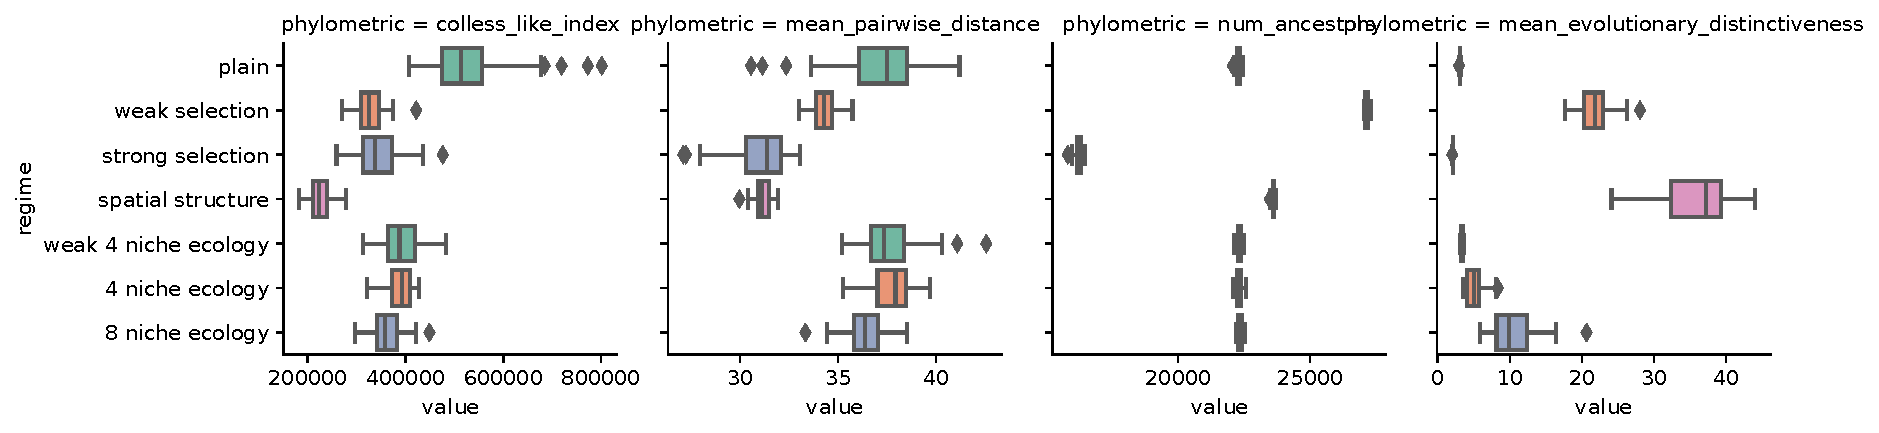
\includegraphics[width=\textwidth]{binder/binder/teeplots/col=phylometric+epoch=7+mut_distn=np.random.standard_normal+viz=boxplot+x=value+y=regime+ext=.pdf}
  % \end{noindent}
  \caption{%
    Distribution of phylometrics measured with perfect phylogenetic tracking across surveyed evolutionary regimes ($n=50$).
  }
  \label{fig:perfect-tree-phylometrics}
\end{teaserfigure}

%%
%% The code below is generated by the tool at http://dl.acm.org/ccs.cfm.
%% Please copy and paste the code instead of the example below.
%%
\begin{CCSXML}
<ccs2012>
   <concept>
       <concept_id>10003752.10003809.10010172</concept_id>
       <concept_desc>Theory of computation~Distributed algorithms</concept_desc>
       <concept_significance>300</concept_significance>
       </concept>
   <concept>
       <concept_id>10010147.10010919.10010172</concept_id>
       <concept_desc>Computing methodologies~Distributed algorithms</concept_desc>
       <concept_significance>300</concept_significance>
       </concept>
   <concept>
       <concept_id>10010147.10010341.10010366.10010369</concept_id>
       <concept_desc>Computing methodologies~Simulation tools</concept_desc>
       <concept_significance>500</concept_significance>
       </concept>
   <concept>
       <concept_id>10010147.10010257.10010293.10011809.10011812</concept_id>
       <concept_desc>Computing methodologies~Genetic algorithms</concept_desc>
       <concept_significance>300</concept_significance>
       </concept>
 </ccs2012>
\end{CCSXML}

\ccsdesc[300]{Theory of computation~Distributed algorithms}
\ccsdesc[300]{Computing methodologies~Distributed algorithms}
\ccsdesc[500]{Computing methodologies~Simulation tools}
\ccsdesc[300]{Computing methodologies~Genetic algorithms}
\maketitle

\vspace{-1.5ex}
\section{Introduction}

Phylogenies (i.e., ancestry trees) reveal how evolving populations move through a search space, which offers a powerful window into understanding the behavior of evolutionary algorithms.
In existing work, phylogenetic analyses have diagnosed conditions stymying adaptive evolution, predicted future adaptive success of evolutionary runs, and revealed the step-by-step process by which an evolutionary algorithm solves a problem \citep{hernandezWhatCanPhylogenetic2022a,shahbandeganUntanglingPhylogeneticDiversity2022a,lalejiniEvolutionaryOriginsPhenotypic2016}.
As evolutionary computation (EC) systems grow in complexity and computational scale  (i.e., parallel and distributed computing), observability enabled through phylogenetic analyses will become increasingly crucial.

Existing phylogenetic methods in EC assume a perfect-tracking model where an exact parentage record enables direct inspection of the lineages without uncertainty or inaccuracy.
Applications to large-scale systems, however, face practical difficulties: communication overhead from record centralization and fragility to data loss.
In contrast, work in biological phylogenetics \textit{estimates} history using extant information from a fully-distributed system.
The recently-introduced ``hereditary stratigraphy'' method facilitates analogous reconstruction-based phylogenetic analysis of distributed EC systems.
This technique works by attaching heritable annotations to individual digital genomes such that trade-off between annotation size and estimation accuracy can be directly tuned \citep{moreno2022hereditary}.

Here, we report follow-up work developing methodological foundations necessary to apply hereditary stratigraphy to observe evolutionary dynamics in complex, distributed digital evolution systems.
First, we characterize the impact of ecology, selection pressure, and spatial structure on phylogenetic metrics.
Second, we quantify the effects of reconstruction-induced estimation error on these phylogenetic metrics.
Third, because distributed methods generally do not support well-mixed populations, we investigate the phylometric signature of interactions of ecology and selection pressure with spatial structure.

\vspace{-1.5ex}
\section{Methods}

Experiments testing the relationships between evolutionary dynamics, reconstruction error, and phylogenetic structure required a model system amenable to direct, interpretable tuning of ecology, spatial structure, and selection pressure.
A parsimonious model system was devised to fulfill these objectives.
Genomes in this system comprised a single floating-point value, with higher magnitude corresponding to higher fitness.
Experiments used the following parameterizations: Gaussian mutation, population size 32,768 ($2^{15}$), 262,144 ($2^{18}$) synchronous generations, and tournament selection.

Treatments explored three evolutionary variables: selection pressure (via tournament size), spatial structure (via an island model with 1D closed-ring topology and 1\% migration rate), ecology (via a simple niche model with niche swap probability $3 \times 10^{-8}$ so one niche swap would be expected every 1,000 generations).
We combined these variables into seven ``regimes'' of evolutionary conditions:

\begin{minipage}[t]{\columnwidth}
\begin{itemize}
  \item \textit{plain}: tournament size 2 with no niching and no islands,
  \item \textit{weak selection}: tournament size 1 with no niching and no islands,
  \item \textit{strong selection}: tournament size 4 with no niching and no islands,
  \item \textit{spatial structure}: tournament size 2 with no niching and 1,024 islands,
  \item \textit{weak 4 niche ecology}: tournament size 2 with 4 niches and niche swap probability increased 100$\times$,
  \item \textit{4 niche ecology}: tournament size 2 with 4 niches, and
  \item \textit{8 niche ecology}: tournament size 8 with 4 niches.
\end{itemize}
\end{minipage}

Sensitivity analysis to evolutionary duration (i.e., number generations) and mutation operator (via an alternate unit-exponential mutation distribution) support our findings' generalizability.

Our phylogenetic analyses employ four metrics: (1) \textit{internal node count}, a measure of phylogenetic richness impacted by ecology and spatial structure; (2) \textit{Colless-like index}, an indicator of tree imbalance associated with varying ecological pressures and spatial structure; (3) \textit{mean pairwise distance}, a metric of evolutionary divergence affected by factors promoting long-term maintenance of distinct branches and factors promoting diversity; and (4) \textit{evolutionary distinctiveness}, another metric of evolutionary divergence calculated at the level of individual taxa --- known to behave differently than mean pairwise distance with a particularly strong relationship to branch length \citep{tuckerGuidePhylogeneticMetrics2017}.

Experiments investigating the impact of phylogenetic inference error on phylometrics test four trade-off levels between resolution and genome annotation size.
Each level is described as a $p\%$ ``resolution'' meaning that uncertainty (generational distance between reference points) $k$ generations back is less than $(p / 100) \times k$. So, a high percentage $p$ indicates coarse resolution and a low percentage $p$ indicates fine resolution.
Annotation size ranged from 68 1-byte fingerprints per genome at coarse 33\% resolution to 1,239 1-byte fingerprints at fine 1\% resolution.

Supporting materials are available at \url{https://osf.io/vtxwd/}.
This project benefited from open-source scientific software \citep{ofria2020empirical,moreno2022hstrat,lalejini2019data,sukumaran2010dendropy}.

\vspace{-1.5ex}
\subsection{Summary of Results}

Each of the four surveyed phylometrics exhibited significant variation between surveyed evolutionary conditions.
Ecological dynamics had a significant but relatively weak influence on phylometrics, suggesting the need to carefully account for selection pressure and spatial structure to ensure accurate detection of ecology through phylogenetic analysis.
The Colless-like index appeared to be less useful for distinguishing evolutionary dynamics: it decreased under all non-plain evolutionary conditions.
Figure \ref{fig:perfect-tree-phylometrics} summarizes the distributions of each phylometric across surveyed evolutionary conditions.

Follow-up experiments tested whether ecological dynamics could still be detected in the presence of spatial structure.
We found this to be the case.
Interestingly, spatial structure appeared to mediate some aspects of ecological phylogenetic structure, which did not appear in its absence.
For instance, ecology had a much larger impact on ancestor count in the presence of spatial structure.
However, spatial structure muted the effects of ecology on the Colless-like index.
These findings highlight the background effects of spatial structure as key to interpretation of phylogenetic signatures of other evolutionary dynamics.

Finally, we analyzed the impact of phylogenetic reconstruction error on phylogenetic analysis.
At the coarsest reconstruction resolution, we detected a significant effect of reconstruction error on all phylometrics except mean evolutionary distinctivenes.
Colless-like index and mean pairwise distance generally reached statistical indistinguishability (at $n=50$) at 3\% reconstruction resolution.
Ancestor count, however, was highly sensitive to reconstruction error.
Future work should investigate the possibility of reducing this sensitivity by resolving polytomies (overrepresented due to reconstruction uncertainty) into sets of bifurcations.
Where detectable, estimation uncertainty bias decreased all surveyed phylometrics' numerical value.
So, when testing for expected increases in phylometric values, the potential for systematic false positives due to reconstruction error can be discounted.

\vspace{-1.5ex}
\section{Conclusion}

Phylogenetic analysis appears feasible means to anatomize complex, distributed evolutionary computing systems.
This work characterizes the phylometric signatures of selection pressure, ecology, spatial population structure, and reconstruction error.
These findings provide a practical, actionable basis for phylogenetic inference of evolutionary dynamics and serves as for starting point for development of a systematic methodology for such analyses.


\vspace{-1.5ex}
\bibliographystyle{ACM-Reference-Format}
\bibliography{bibl} % replace by the name of your .bib file

\end{document}
